\documentclass[CSHFoundation.tex]{subfiles}
\begin{document}



\chapter{Home}
\centerline{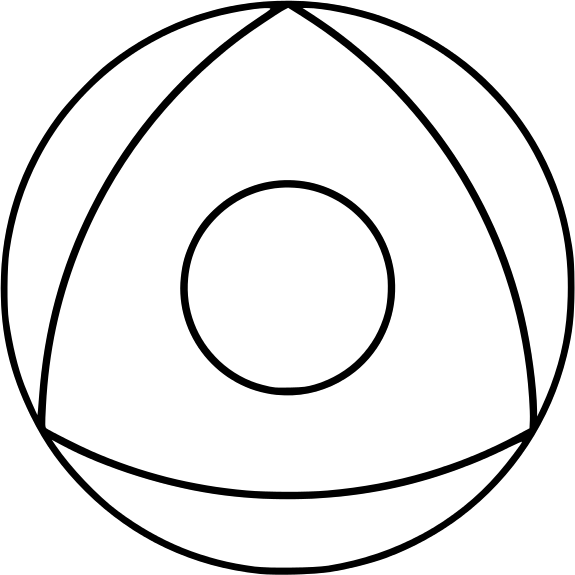
\includegraphics[scale=0.35]{6-Hlogo.png}}
\section{Home Constitution}

\subsection{Purpose}

Planet Home’s focus is on establishing healthy, thriving families. This is established by the physical support, mental support, and spiritual support that parents offer to their children through relationship.


\subsection{Roles}

\subsubsection{Mothers}

Mothers provide the physical, emotionally, and genetic support that a child needs at their earliest stages. A child cannot function without a mother for the first nine months of their life. It is in the best interest of the child therefore, the maintain this connection for the rest of their life. In the case of a dysfunctional family: Planet Home seeks rather to help the original mother of the child find help in raising a child, rather then to remove the child from the situation. However, if the mother is unwilling to change, measures might need to be taken to provide a safe home for the child. A mothers role is to work with the resources to create a place where others can thrive.

\subsubsection{Fathers}



As a child also cannot be created without the help of a father, and genetic code is passed from father to child, it is imperative that a child know their father. It is also crucial that a father spend time with their child, and show their love to them. Love of a father prevents many emotional problems later in life. A fathers role is to provide the physical resources needed for the home.



\subsubsection{Younger Children (\textgreater{}=12)}



Younger children cannot care for themselves fully, and need supervision. Food, Water, and Sleep are not enough for these children to thrive. They need to have security, fun, and love in addition to grow.



\subsubsection{Older Children (\textless{}12)}



Middle children represent a key transformation period. They go from playing with toys, to playing with real life. No longer are their amusements purely theoretical, but they transfer into situations that have significant consequences. It is at this point that the child is given more and more privileges to aid in their maturity development. In addition, they might be required to care for younger children as well, or work to help provide for the families income.



\subsection{Layout}



\subsubsection{Co-Ed Family}



A family should not consist of more then 12 individuals, with a mother figure and a father figure. It is ideal [if not mandatory], that this couple be married. In planet Home a family name is given to those who belong to a family. It is recommended children keep their original last name, however, substituting it as a middle name. This family is for life, and the kids will be legally adopted as children of the new parents. It is not recommended that these parents take more then 12 children during their time as parents, as these connections should be built for life. The more connections, the less time can be given to each individual. This base unit of a family is designed to eat together, often play together, and live alongside each other. A Family should consist of both boys and girls, however, extreme care must be given. If children are raised alongside each other from a young age, there will be significantly less sexual attraction. Well functioning family should be the safest place to be, for there must be much love.



\subsubsection{Single Gender Family}



A separate contingent of family groups will be established for the development of kids who enter into Planet Home at a later age (10 and up). These children still need all the love and support that the Co-Ed Family’s provide, and so the structure will be identical, with the exception that this family has only one gender.



\subsubsection{Mentorship Family}



It may come that a boy or a girl comes to planet Home needing help, however, as they are already over the age of 16, and feel a strong need for independence, forcing a family upon them might have a detrimental effect. What they need is help, but not things handed to them, for they are already at a place in life where they can provide for themselves. A mentorship family provides the love and support necessary to build these children up, without forcing a family they do not know on them. Could be run by a single person (same gender as mentoree)



\subsection{Functions}



\subsubsection{Marriage}



Marriage marks the beginning of a new family, and should not be discouraged for the older children. The new couple then will have to leave Planet Home, and start a new family somewhere else (hopefully reasonable living quarters can be provided for). This breaks the cycle of physical poverty given to these children, and allows them with a solid foundation to start a new life. There is no age limit on marriage, but rather a focus on maturity of the individuals to spend their life together. The host parents need to be involved in the establishment of this new marriage, providing counsel for the newly-weds. All those wishing to get married must have the firm mindset that marriage is forever. A marriage ceremony should be conducted without going into debt. As many newlyweds do not have the funds, parents will offer to pay for parts of the wedding.



\subsubsection{Family}



It is important to have homes in the context of family. Individual homes should make an effort to meet with family members often. For those who do not have family, homes will be paired with homes for the purpose of family.



\subsubsection{Friends}



Children also need to have friends, and having families interact with each other brings about an opportunity for kids to meet and play with other kids.



\subsubsection{Physical Needs}



Home provides not only the physical needs of a child, but the training of children in physical safety, rest, relaxation, exercise, etc.



\subsection{Integration}



\subsubsection{Church}



Students should be provided with spiritual instruction, however, it should not be the role of those with the spiritual gift of teaching to teach those students. Families have the obligation to teach their children much of what the Bible says, from praying before meals, to doing devotions at night, but a child also needs to be with other believers who commonly meet together. It is this environment that provides the growth needed to transform a new Christian into a strong Christian. A family must make the attempt to continue to meet with other believers regularly for the purpose of spiritual growth. This is accomplished by the core group in church. A single family meets with other families to compose this group. Meeting regularly, they encourage each other in life.



\subsubsection{School}



School is a must for all kids, and all students go to school.



Children should be taught by their parents or family member until the age of 11. If this is an impossibility, the school does provide education at the facility, but it is with involvement from parents attending a church.

\section{Dating}


\subsection{Purpose}

Dating is the process in which to find a life-long mate

\subsection{Procedure}

The aspiring man/woman has 3 options:

\begin{itemize}
\item Option 1: Ask their parents to find a mate
\item Option 2: (male) Look for a mate on their own
\item Option 3:Aspire to live a life of singleness until further notice
\end{itemize}

\subsubsection{Option 1}

The parents of the man, in collaboration with the parents of the woman, bring the couple together. The couple is both under the assumption that the other is looking for a marriage partner. After a maximum of 3 months, the man/woman must decide if this is the woman he/she wants to marry, and the man must propose. At this point the relationship moves into the Engagement stage.



\subsubsection{Option 2}

The man  looks for a future spouse on his own. Once he has found a potential wife, he must get approval from her parents, and his parents before going on the first date. At this point the same method follows as Option 1.



\subsubsection{Option 3}

A man or woman seeking to be devoted to the Lords Work may desire to not seek a wife or husband. They must not be condemned as forsaking the raising of children, for their mission is now to raise the children of God.



\subsubsection{Codes of Conduct}

During these periods, the man should refrain from physical interaction as much as possible, so that the marriage day may be the first time the couple touch.

To further push this policy: all dates must be in open places. Dates cannot be held in personal rooms, or in houses with no one home. Treat the other as you would a brother or sister.



Sex before marriage is absolutely prohibited, as it shames the image of the union between Christ and His Church. Those who cannot wait are encouraged to marry quickly.\footnote{1 Corinthians 7:9}

\section{Wedding}



\subsection{Definition}

Marriage is a joining of a man and a woman to become one flesh, applying to physical, emotional, intellectual, and spiritual intimacy. It is the process in which two separate individuals become one. As one cannot separate himself, marriage reflects a life-long commitment. Marriage has not happened until this commitment is made public.


\subsection{Process}
\subsubsection{Part 1: Engagement}

The man promises himself to the woman, and she wears a symbol of his love. He also wears the same symbol.\footnote{This is not to say that all marriages should proceed. This is simply an example to emphasize the picture of Christ and His Church} They both sign the certificate for marriage on this day, agreeing to love each other, and have it signed by the bride's parents as well.  For the remainder of this time, she no longer has any contact with him. This phase should take at a maximum 3 months. At the final day, she will wait. Not knowing the hour, but waiting until he comes. When he does come, the ceremony will begin. Breaking this agreement is par with divorce.



\subsubsection{Part 2: Coming}

The man, along with the guests of the party, arrive at the bride's house, and walk over with singing to the groom's house. The groom, along with the bridal party, escort the bride and groom to their new home, where the marriage is consummated.\footnote{This emphasizes the fact the couple has been waiting for sexual intimacy until their declaration of love before a community. It also acknowledges that sexual intimacy is part of becoming one flesh. Some may be incapable of sexual intimacy for biological reasons. This does not mean they are not married. However, for those that can, should recognize that sexual intimacy is important to the process}



\subsubsection{Part 3: Party}

The party returns, joyful, and the party begins. This is meant to be a relaxing party, with stories, dancing, singing, and at the very end, the Lords supper, and a reminder that we wait his return.


The bridal party are the witnesses to the marriage, and they pledge to help the new couple in their marriage.



\subsection{Remarks:}

\begin{itemize}
\item this can happen outside of a religious building.
\item Far cheaper
\item Bride and Groom wear matching white robes, can change later
\item The parents off to pay for parts of the wedding, and possibly  honeymoon.\footnote{New couples should not be worrying about the expenses of a wedding during this time. This is meant as a celebration, and a welcome into the next chapter of their lives. To go into debt for a wedding is financially wrong}
\end{itemize}

\section{Marriage}
\subsection{Purpose}
Marriage is a reflection of Christs relationship to His church. Relationships are more then a one time event, it takes a lifetime of learning and growth. There is a danger for couples to grow cold to each other, to forget their commitment, and leave each other, for the destruction of their children and themselves. The Home organization, in partnership with the church and school, is committed to helping couples maintain this relationship

\subsection{Foundation}
According to the Fundamental Belief of relationship:

\begin{enumerate}
\item Relationship requires exploration
\item Relationship requires physical interaction
\item Relationship requires giving of ourselves
\item Relationship requires commitment
\item Relationship requires communication
\item Relationship requires submission to each other
\item Relationship requires change and repentance
\item Relationship requires living life together
\item Relationship requires love
\end{enumerate}

\subsection{Theory}
To this end:

Couples should

\begin{enumerate}
\item Purposefully explore each other (spiritually, emotionally, intellectually, physically)
\item Touch each other (skin to skin), and be around each other after work.
\item Take time to do something the other 
\end{enumerate}desires

\begin{enumerate}
\item Be committed to each other
\item Communicate with each other about how they are doing (and how their relationship is going)
\item Submit to one 
\end{enumerate}another

\begin{enumerate}
\item Change when something is wrong with the relationship
\item Live life together (in the same bed, at the same table, in the same house)
\item Love each other
\end{enumerate}

\subsection{Practice}

\begin{itemize}
\item Daily: The couple spends time to go over how the day went, and how they feel
\item Weekly: the couple spends an evening all by themselves (one week the wife chooses, the next, the husband)
\item Monthly: the couple spends a full night without the kids being there (can be merged with a weekly date night)
\item Yearly: A week getaway where the couple brings enough food, but no telecommunication.
\end{itemize}

\section{Education}

Home will also implement the levels approach to educating kids. It is the parents responsibility, and not the teachers, to develop moral citizens. This is a loose guide for parents to follow. Students will not be tested on the following, but it is the parents responsibility to educate their own kids. The school will check in on parents to see how things are going, and provide them with resources as needed.



\subsection{Health \$ Safety}

\begin{enumerate}
\item Eating right (5 levels)
\item Sleeping
\item Staying safe outside
\item Relationships
\item Time management
\item Stress
\item Habits
\item Marriage \$ Sex
\end{enumerate}

\section{Floor Plans}

The idea behind communal living is such:

\begin{itemize}
\item Cheaper upkeep (as less surface area exposed to outside)
\item Housing for new families (in the context of friends / families)
\begin{itemize}
	\item (Thus making marraige a possibility for those who are not well to do financially)
\end{itemize}\item Community focus, brings people together (not apart)
\item Large gathering areas for social functions (ie: church services)
\end{itemize}

Each unit can be customized for which types of floors it encorperates



The expected housing capacity is as follows:

\begin{itemize}
\item Large - 8 * 6 apartments = 48 people
\item Medium - 6 * 12 = 60 people
\item Small -  4 * 16 = 64 people
\end{itemize}

There is no expected elevator, making 4 floors an logical limit (for a maximum capacity then of  256 people)

\begin{center}
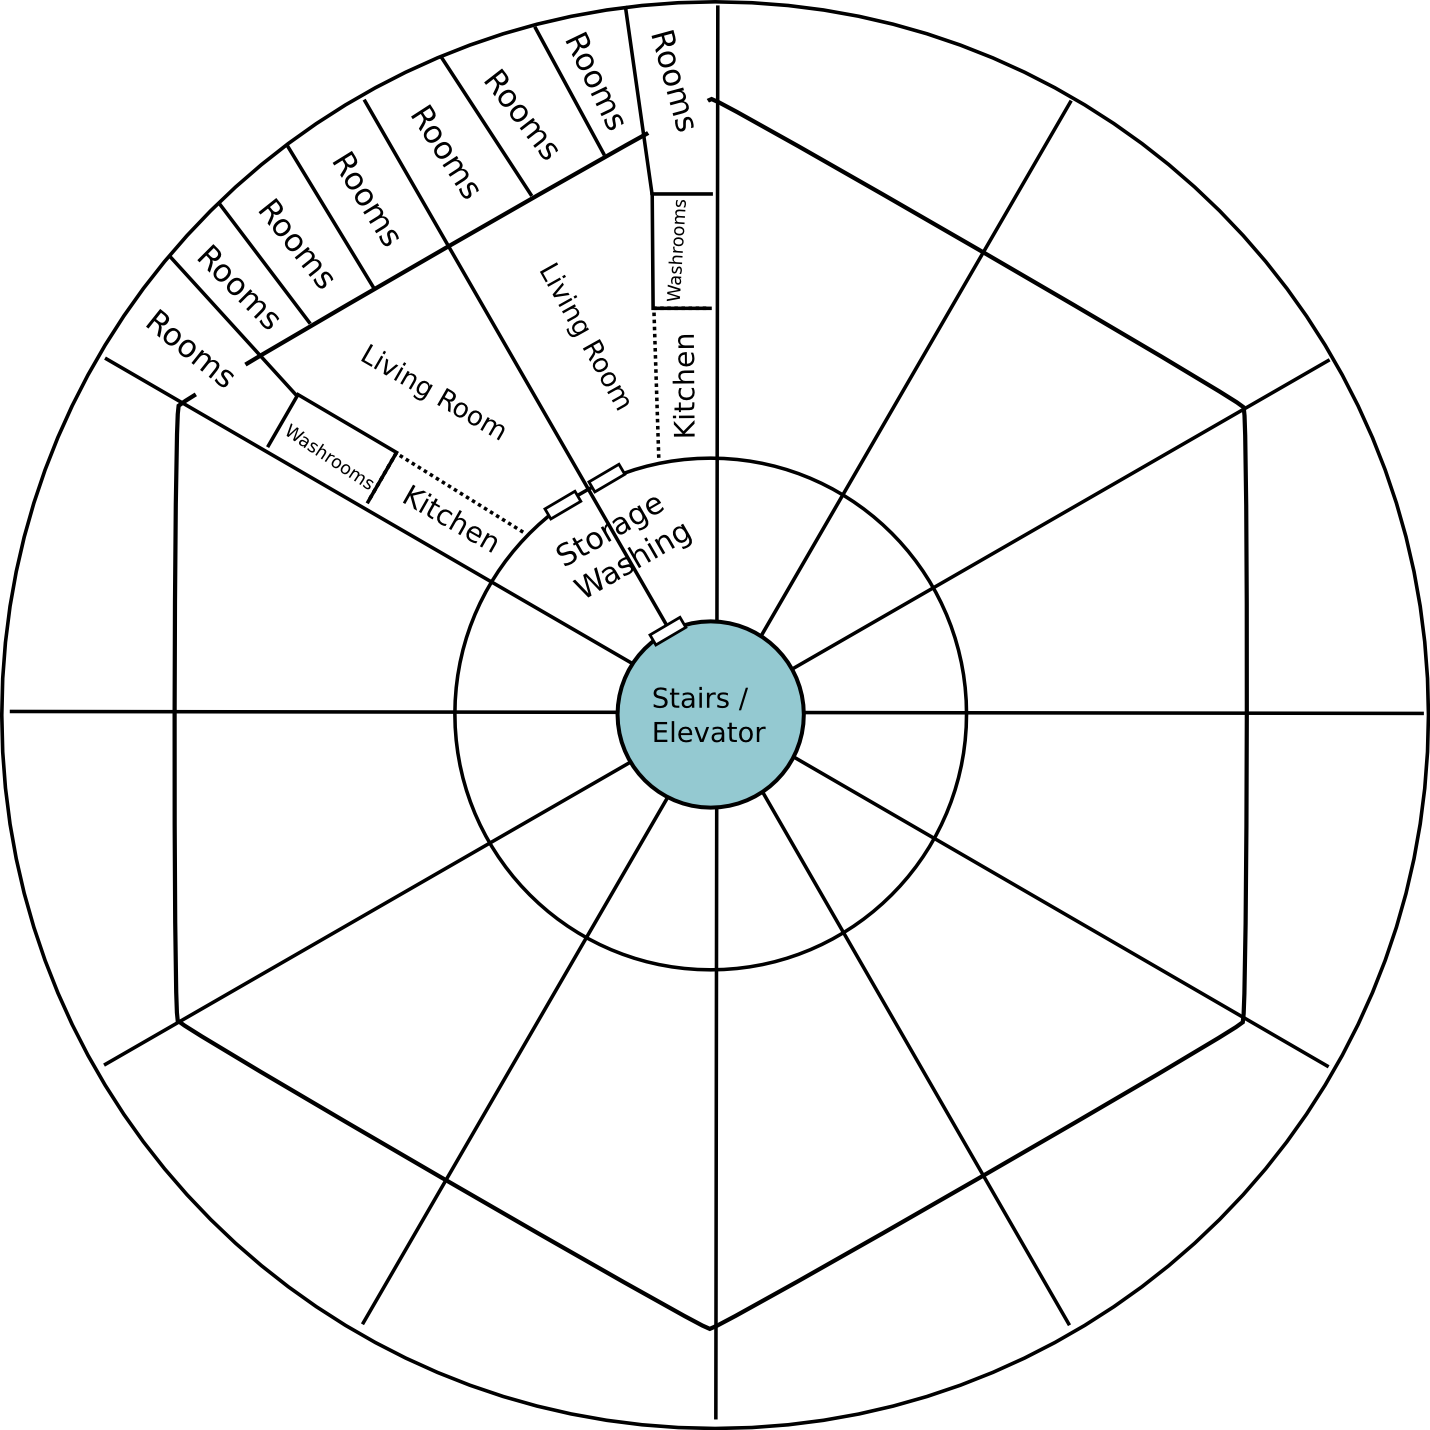
\includegraphics[scale=0.4]{3-community home dorms.png}
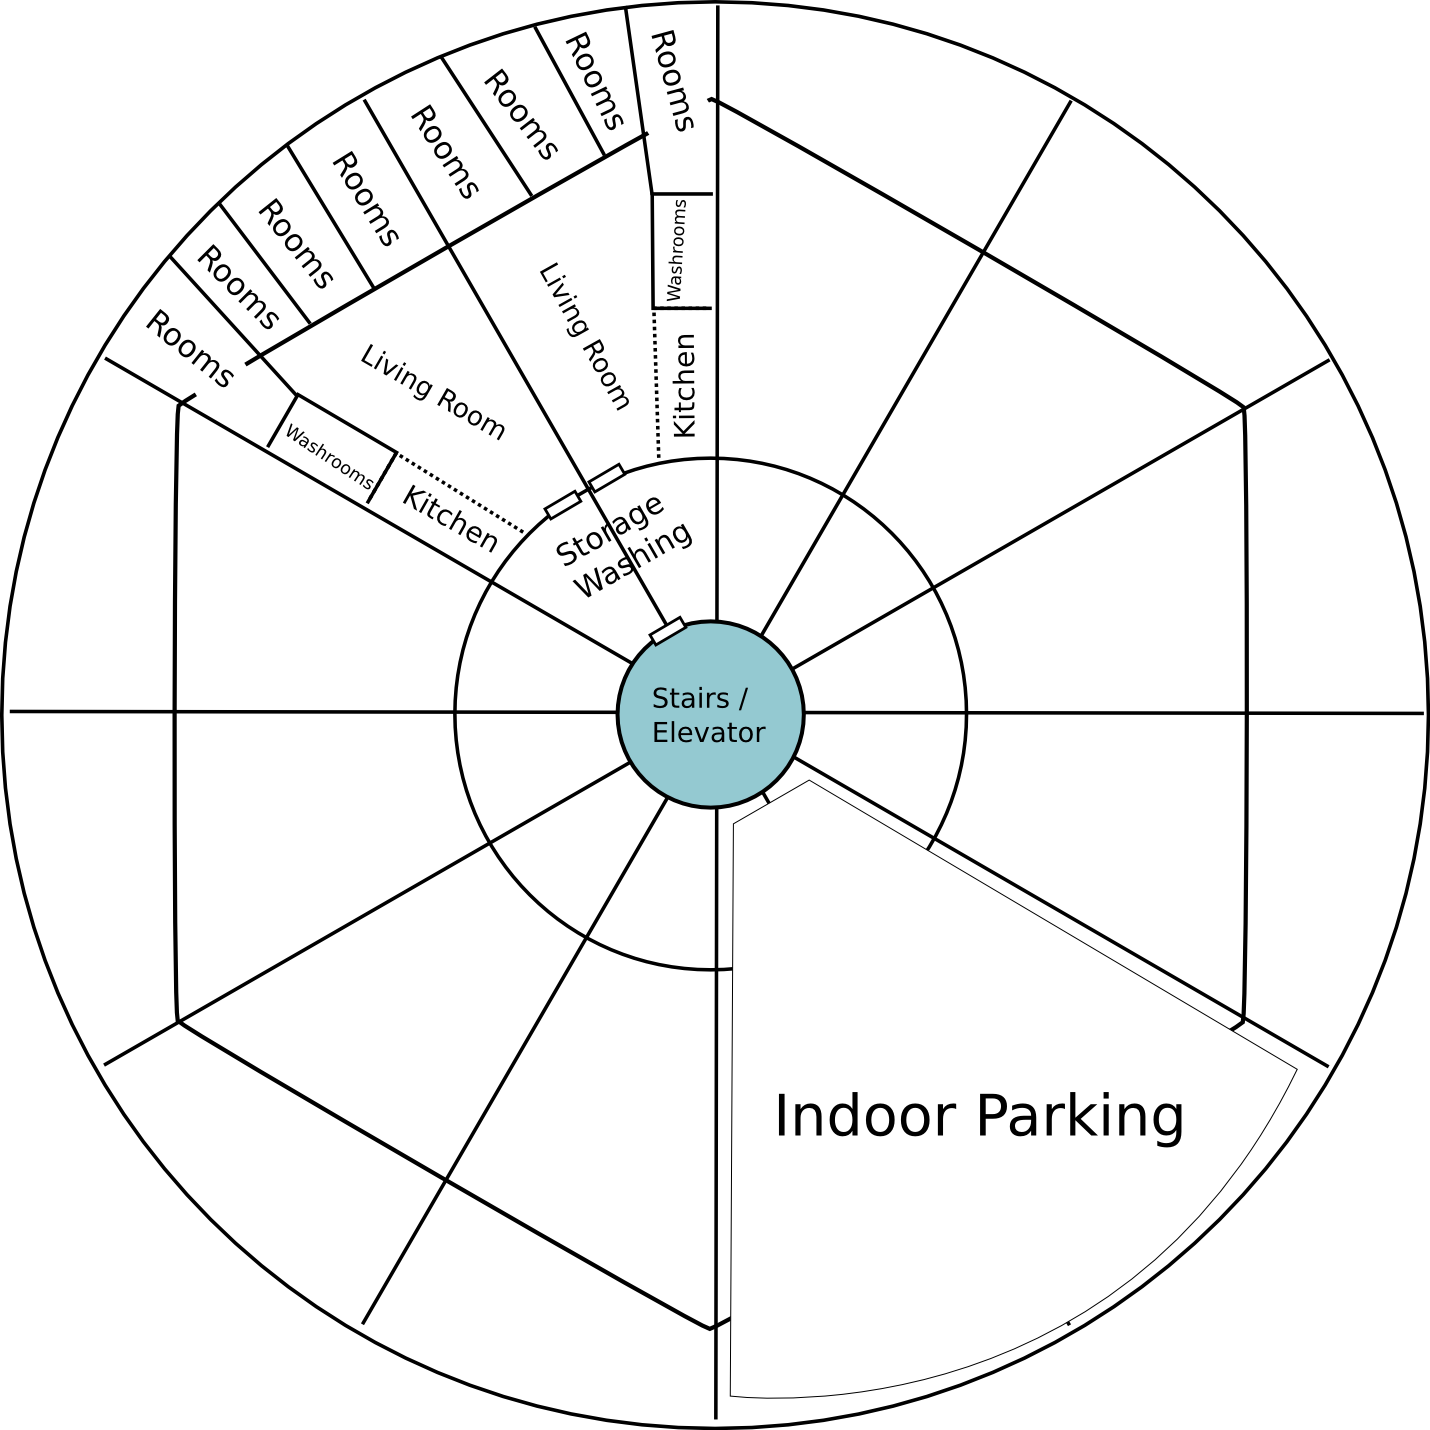
\includegraphics[scale=0.4]{3-community home entry housing.png}
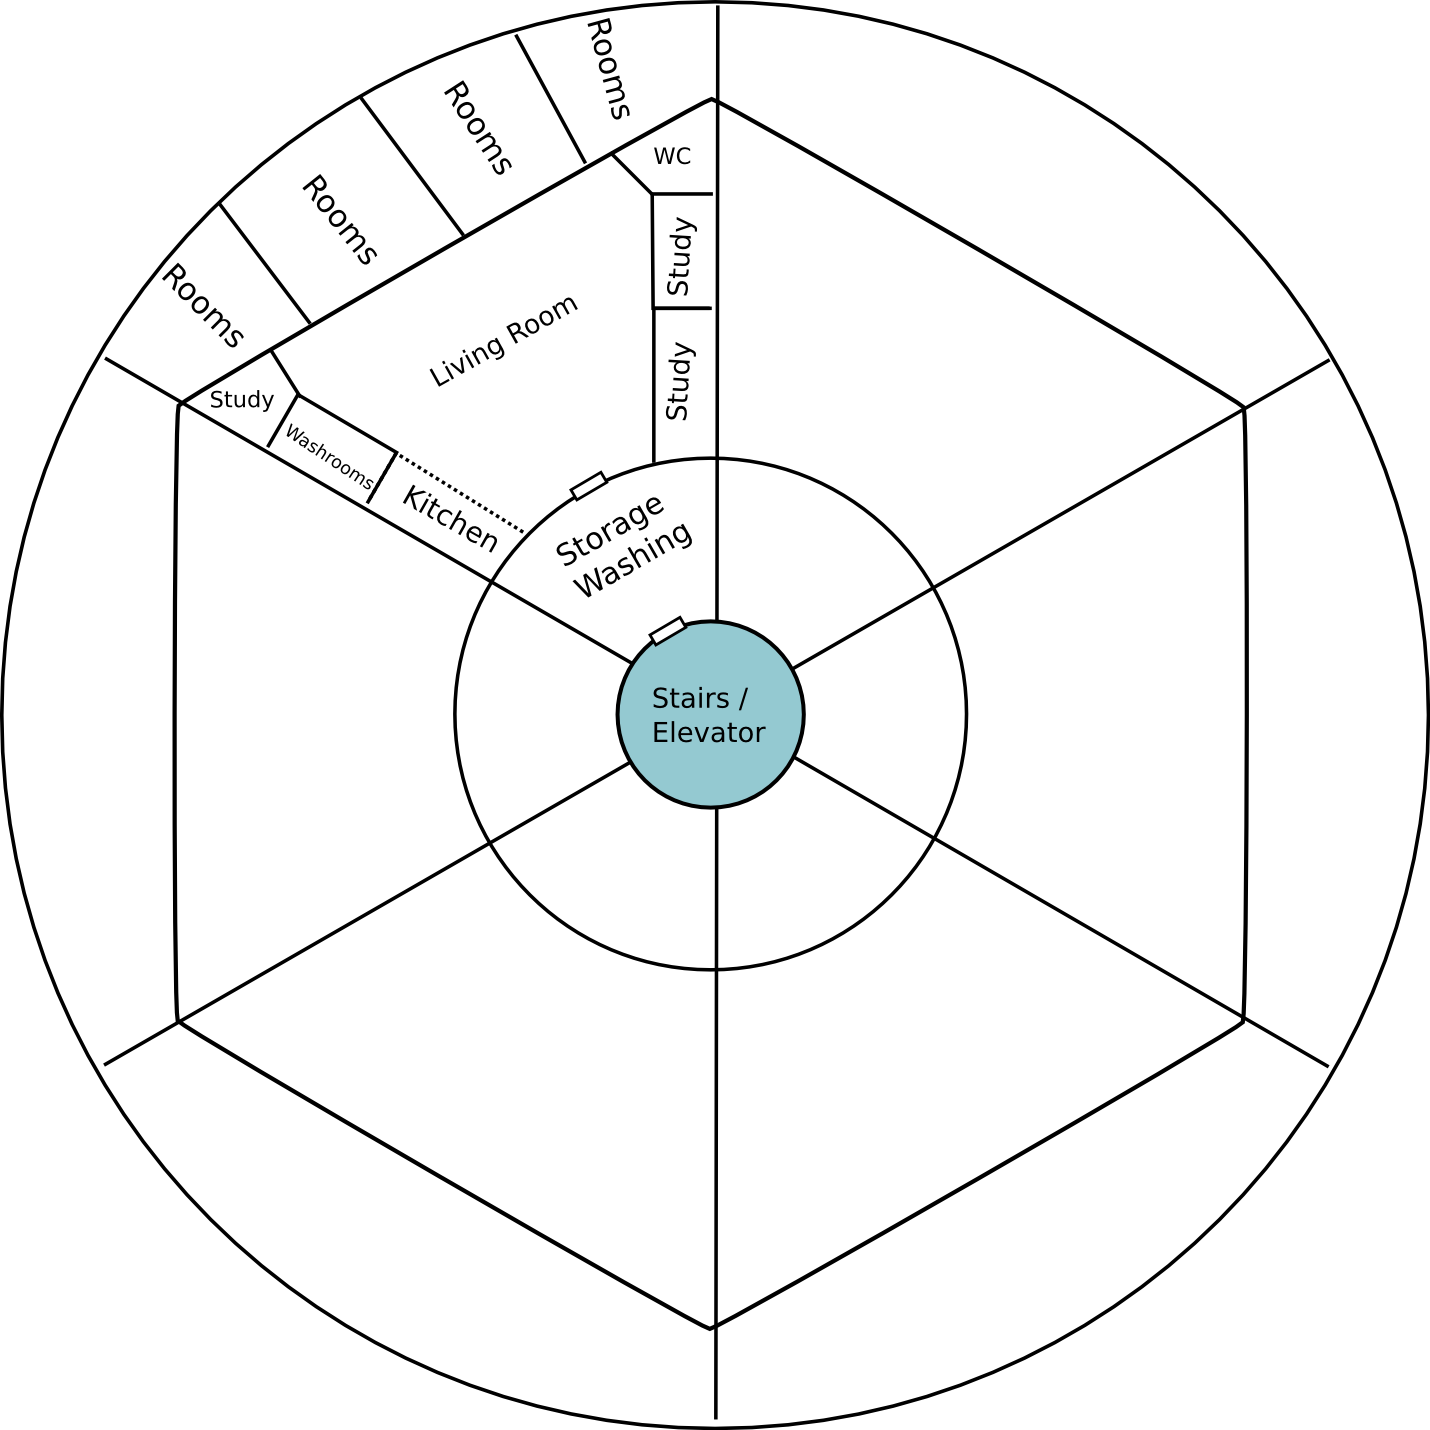
\includegraphics[scale=0.4]{3-community home large.png}
\end{center}

\end{document}